% chapters/chapter3/3_4_nmpc_basic.tex
% !TeX root=../../main.tex

\section{ارزیابی \lr{NMPC} در تنظیم نقطه ثابت}
\label{sec:nmpc_basic_analysis}

در این بخش، عملکرد کنترل‌کننده پیش‌بین مدل غیرخطی (\lr{NMPC}) در غیاب برنامه‌ریز مسیر و در مواجهه مستقیم با خطای موقعیت (ورودی پله) ارزیابی می‌شود. هدف از این تحلیل، بررسی توانایی الگوریتم بهینه‌ساز در مدیریت هم‌زمان خطاهای بزرگ، ارضای قیود سخت فیزیکی و بهره‌گیری از عملگر وینچ در شرایطی است که هیچ‌گونه مسیر مرجع همواری برای هدایت سیستم وجود ندارد.

\subsection{مانور کوتاه‌برد}
در مانور کوتاه‌برد (شکل~\ref{fig:nmpc_step_05_analytical})، خطای اولیه کالسکه در مسافت $0.5$ متر تنظیم شده است. به دلیل کوچک بودن این خطا، سیستم رفتار نسبتاً ملایمی از خود نشان می‌دهد. زاویه نوسان آونگ در بیشینه خود به حدود $0.11$ رادیان می‌رسد که فاصله امنی تا مرز قید سخت فیزیکی ($15^\circ$ معادل $\pm0.26$ رادیان) دارد.

تلاش کنترلی در این سناریو (نیروی کالسکه و شتاب وینچ) بسیار هموار و محدود است. در این شرایط، درجه آزادی کابل ($\ddot{l}$) تقریباً غیرفعال باقی می‌ماند؛ زیرا انرژی ارتعاشی قابل‌توجهی تولید نشده است که حل‌گر را ملزم به فعال‌سازی مکانیزم میرایی کابل کند. با این حال، کالسکه در فرآیند رسیدن به مبدأ با یک فراجهش در موقعیت مواجه می‌شود که ناشی از تنظیمات وزن‌دهی بهینه‌ساز (کاهش وزن ردیابی موقعیت به نفع مهار نوسان) است.

\begin{figure}[htbp]
    \centering
    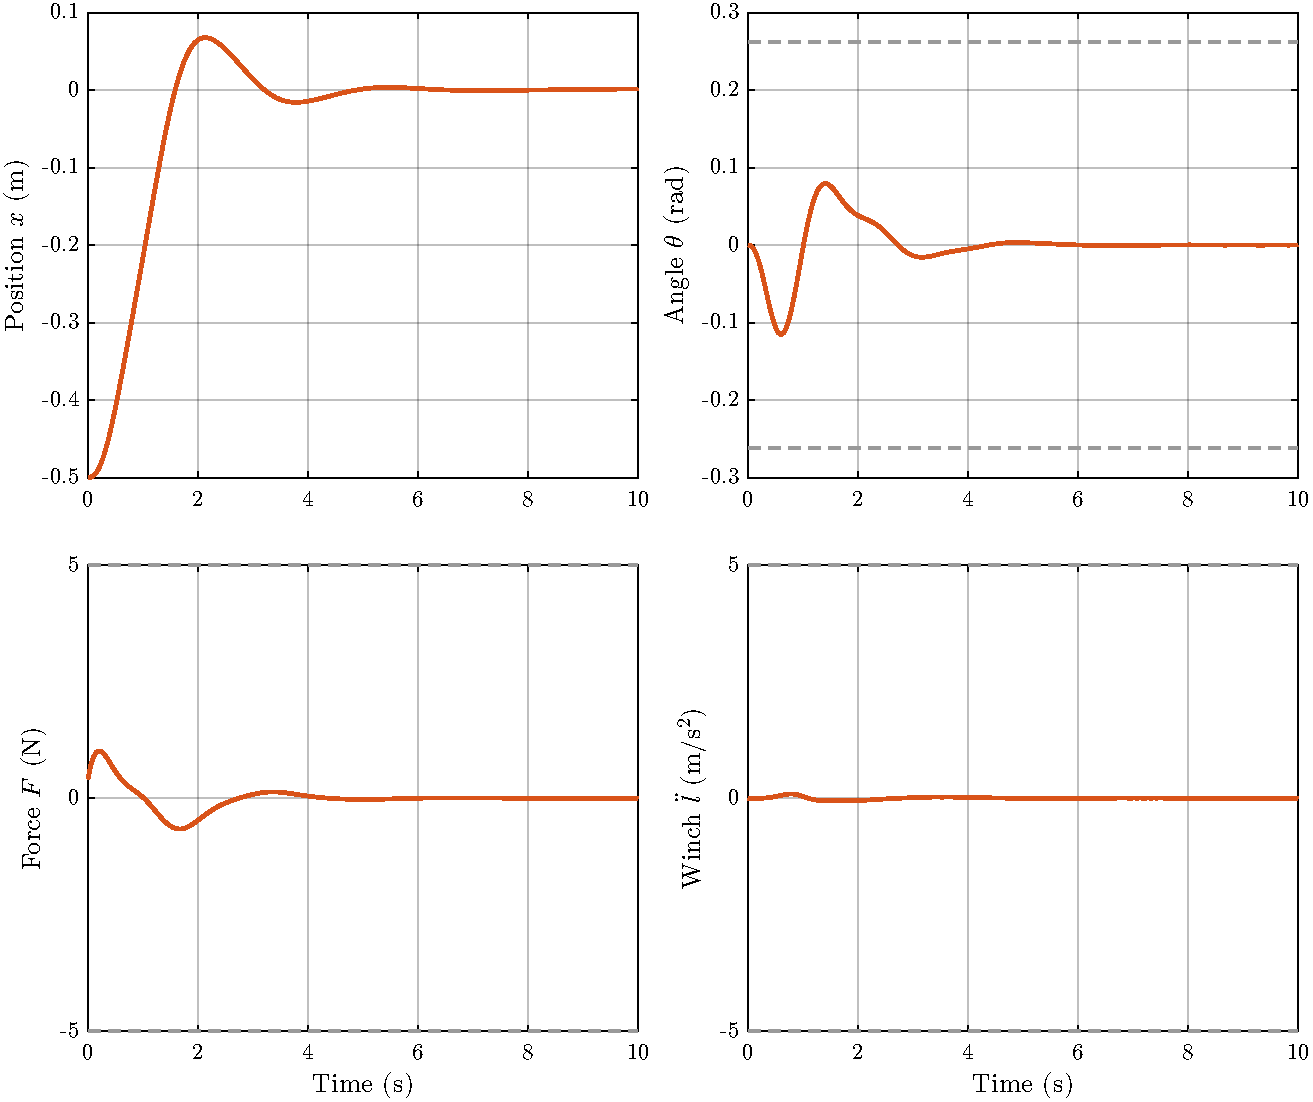
\includegraphics[width=0.85\textwidth]{images/3_NMPC_Basic/NMPC_Basic_Analytical_05.pdf}
    \caption{\rl{پاسخ زمانی متغیرهای حالت و تلاش کنترلی در مانور کوتاه‌برد ($0.5$ متر) تحت کنترل‌کننده \lr{NMPC} در ردیابی پله.}}
    \label{fig:nmpc_step_05_analytical}
\end{figure}

\subsection{مانور بلندبرد و اثر فقدان مسیر مرجع}
چالش اساسی در مانور بلندبرد $5$ متری (شکل~\ref{fig:nmpc_step_5_analytical}) بروز می‌یابد. فقدان یک مسیر مرجع پیوسته (\lr{Trajectory}) سبب می‌شود تا کنترل‌کننده در لحظه آغازین با یک خطای موقعیت بسیار بزرگ روبه‌رو شود. حل‌گر \lr{NMPC} برای کمینه کردن سریع این خطای پله، فرمان شتاب‌گیری شدیدی صادر می‌کند که سیستم را سریعاً به مرزهای قیود فیزیکی خود می‌راند.

همان‌طور که در نمودار زاویه آونگ مشهود است، پاندول در همان ثانیه‌های نخست به کران‌های مجاز خود ($0.26$ و $-0.26$ رادیان) برخورد کرده و به شدت روی این مرزها حرکت می‌کند. برای حفظ آونگ در این محدوده مجاز و جلوگیری از نقض قید در حین حرکت سریع کالسکه، کنترل‌کننده مجبور به مداخله‌های شدید، متناوب و تهاجمی می‌شود. این امر به وضوح در نمودارهای تلاش کنترلی قابل مشاهده است؛ نیروی اعمالی به ارابه ($F$) و شتاب وینچ ($\ddot{l}$) دچار نوسانات شدید و تغییرات فرکانس بالا شده‌اند تا تعادل سیستم در مجاورت مرزها حفظ شود.

علاوه بر نوسانات شدید عملگرها، دینامیک موقعیت نیز دچار اختلال می‌شود. کالسکه به جای توقف نرم در مبدأ، یک فراجهش مهارنشدنی و بسیار بزرگ (حدود $1.5$ متر) را تجربه می‌کند و پس از رفت و برگشت‌های متوالی در حدود ثانیه $8$ به پایداری نسبی می‌رسد.

\begin{figure}[htbp]
    \centering
    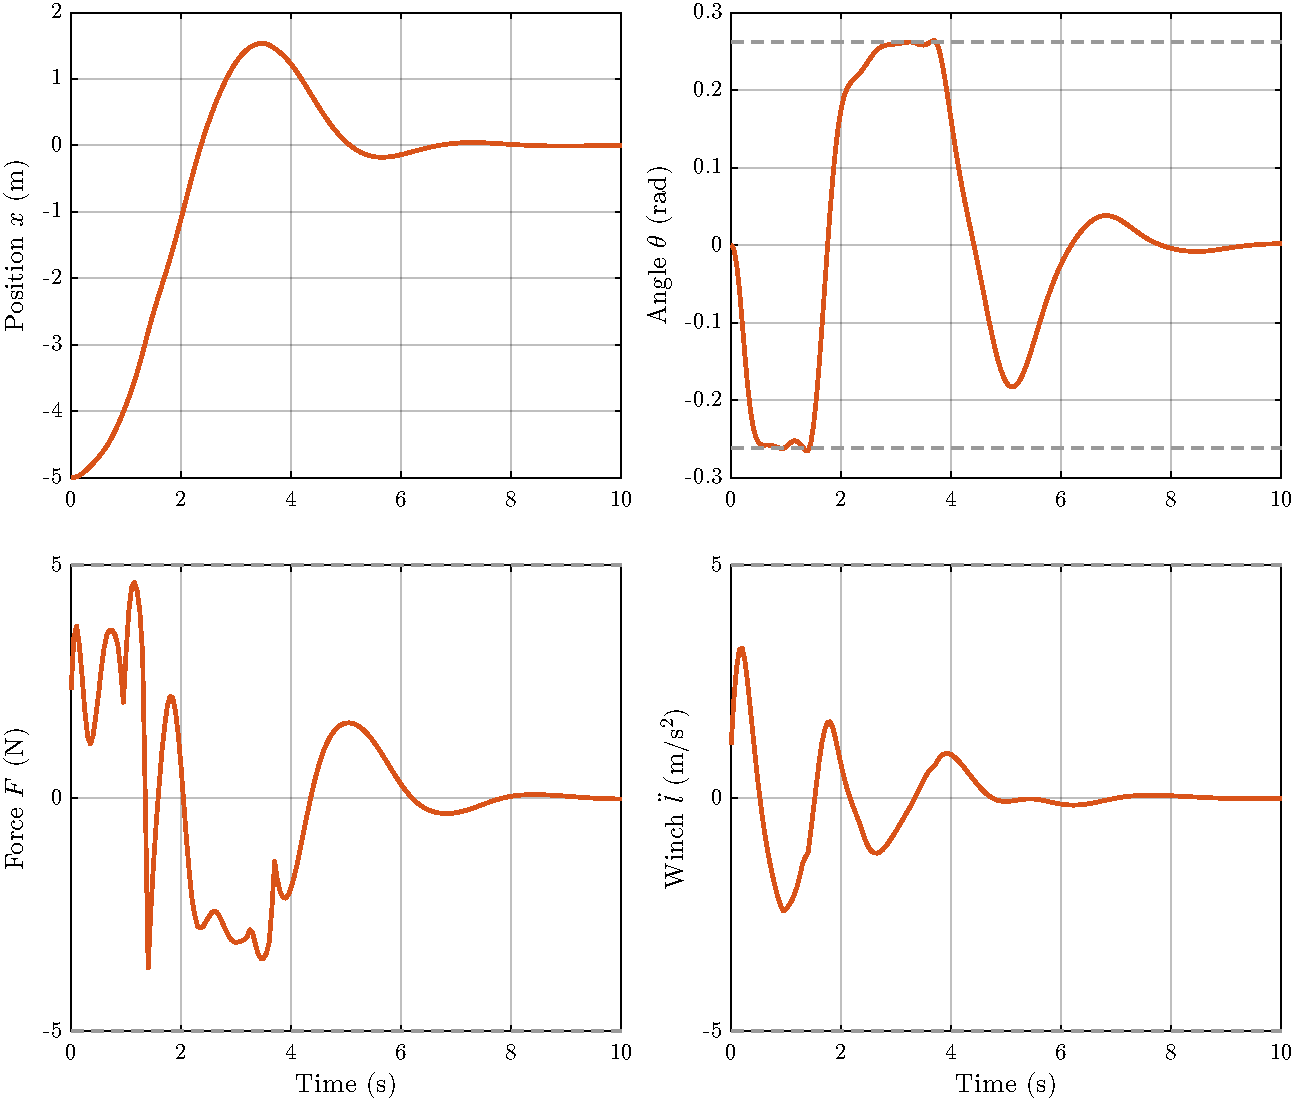
\includegraphics[width=0.85\textwidth]{images/3_NMPC_Basic/NMPC_Basic_Analytical_5.pdf}
    \caption{\rl{پاسخ زمانی سیستم در مانور بلندبرد ($5$ متر)؛ درگیری شدید با مرزهای قید، فراجهش موقعیت و نوسانات نامطلوب در تلاش کنترلی.}}
    \label{fig:nmpc_step_5_analytical}
\end{figure}

\subsection{مصالحه میان نرمی کنترل و دقت ردیابی}
رفتار مشاهده‌شده در سناریوی بلندبرد ثابت می‌کند که اگرچه معماری پیش‌بین غیرخطی قادر است با فعال‌سازی درجات آزادی خود از چرخش آونگ و فروپاشی کامل دینامیکی (که در \lr{LQR} رخ داد) جلوگیری کند، اما استفاده از آن به عنوان یک تنظیم‌گر نقطه ثابت مطلوب نیست.

درگیری سریع و ممتد سیستم با مرزهای قید زاویه، منجر به تولید فرامین کنترلی نوسانی و خشن روی نیروی اعمالی ارابه می‌شود. این نوسانات متناوب در سیگنال‌های کنترلی، علاوه بر کاهش دقت ردیابی موقعیت، از منظر مهندسی سبب افزایش شدید استهلاک مکانیکی و تحریک دینامیک‌های مدل‌نشده سازه خواهد شد. این مشاهدات نتیجه‌گیری می‌کند که برای مهار ایمن سیستم و دستیابی به تلاش کنترلی نرم، تزریق یک مسیر سینماتیکی به افق پیش‌بینی \lr{NMPC} یک ضرورت قطعی است.